\chapter{Conclusions}\label{ch:Conclusions}
In the era of neutrino precision measurements, of huge liquid argon detectors and of massive amount of information from LArTPCs, a renewed interest for an ancient measurement arises: the measurement of hadronic interactions with matter. With this work, we presented the first ever ($\pi^-$-Ar) and ($K^+$-Ar) total hadronic cross section measurements as a function of the hadron kinetic energy. These analyses are the first physics analyses developed by the LArIAT experiment.
Both the analysis follow a similar workflow and  they rely on beam line detector information as well as both calorimetry and tracking in the TPC. 


In order to measure ($\pi^-$-Ar) total hadronic  argon cross sections, we start by selecting pion beamline candidates through a series of selections on the beamline and TPC information apt to maximize the number of pions in the selection over the number of muons and electrons. We use the LArIAT beamline MC to estimate the beam composition of the selected beamline candidates and we propagate them to the LArAIT TPC constructing a properly weighted sample with the DDMC. We apply the thin slice method on the pion candidates and obtain the raw cross section measurement. From the simulated sample, we obtain two corrections accounting for the beamline background contamination and for detector effects. Finally, we apply the corrections to data and measure the true cross section.

In order to measure ($K^+$-Ar) total hadronic  argon cross sections, we follow a similar procedure, i.e. we apply the thin slice method on kaon candidates identified in the beamline to obtain the raw cross section. We apply a background correction and a correction for detector effects to the raw cross section.
The background correction accounts for the presence of secondary particles in both the interacting and incident histograms and for the presence of decay events in the interacting plot.

The final results for the ($\pi^-$-Ar) and ($K^+$-Ar) total hadronic cross section are shown side by side in figure \ref{fig:finalfinal}.

\begin{figure}[htb]
\centering
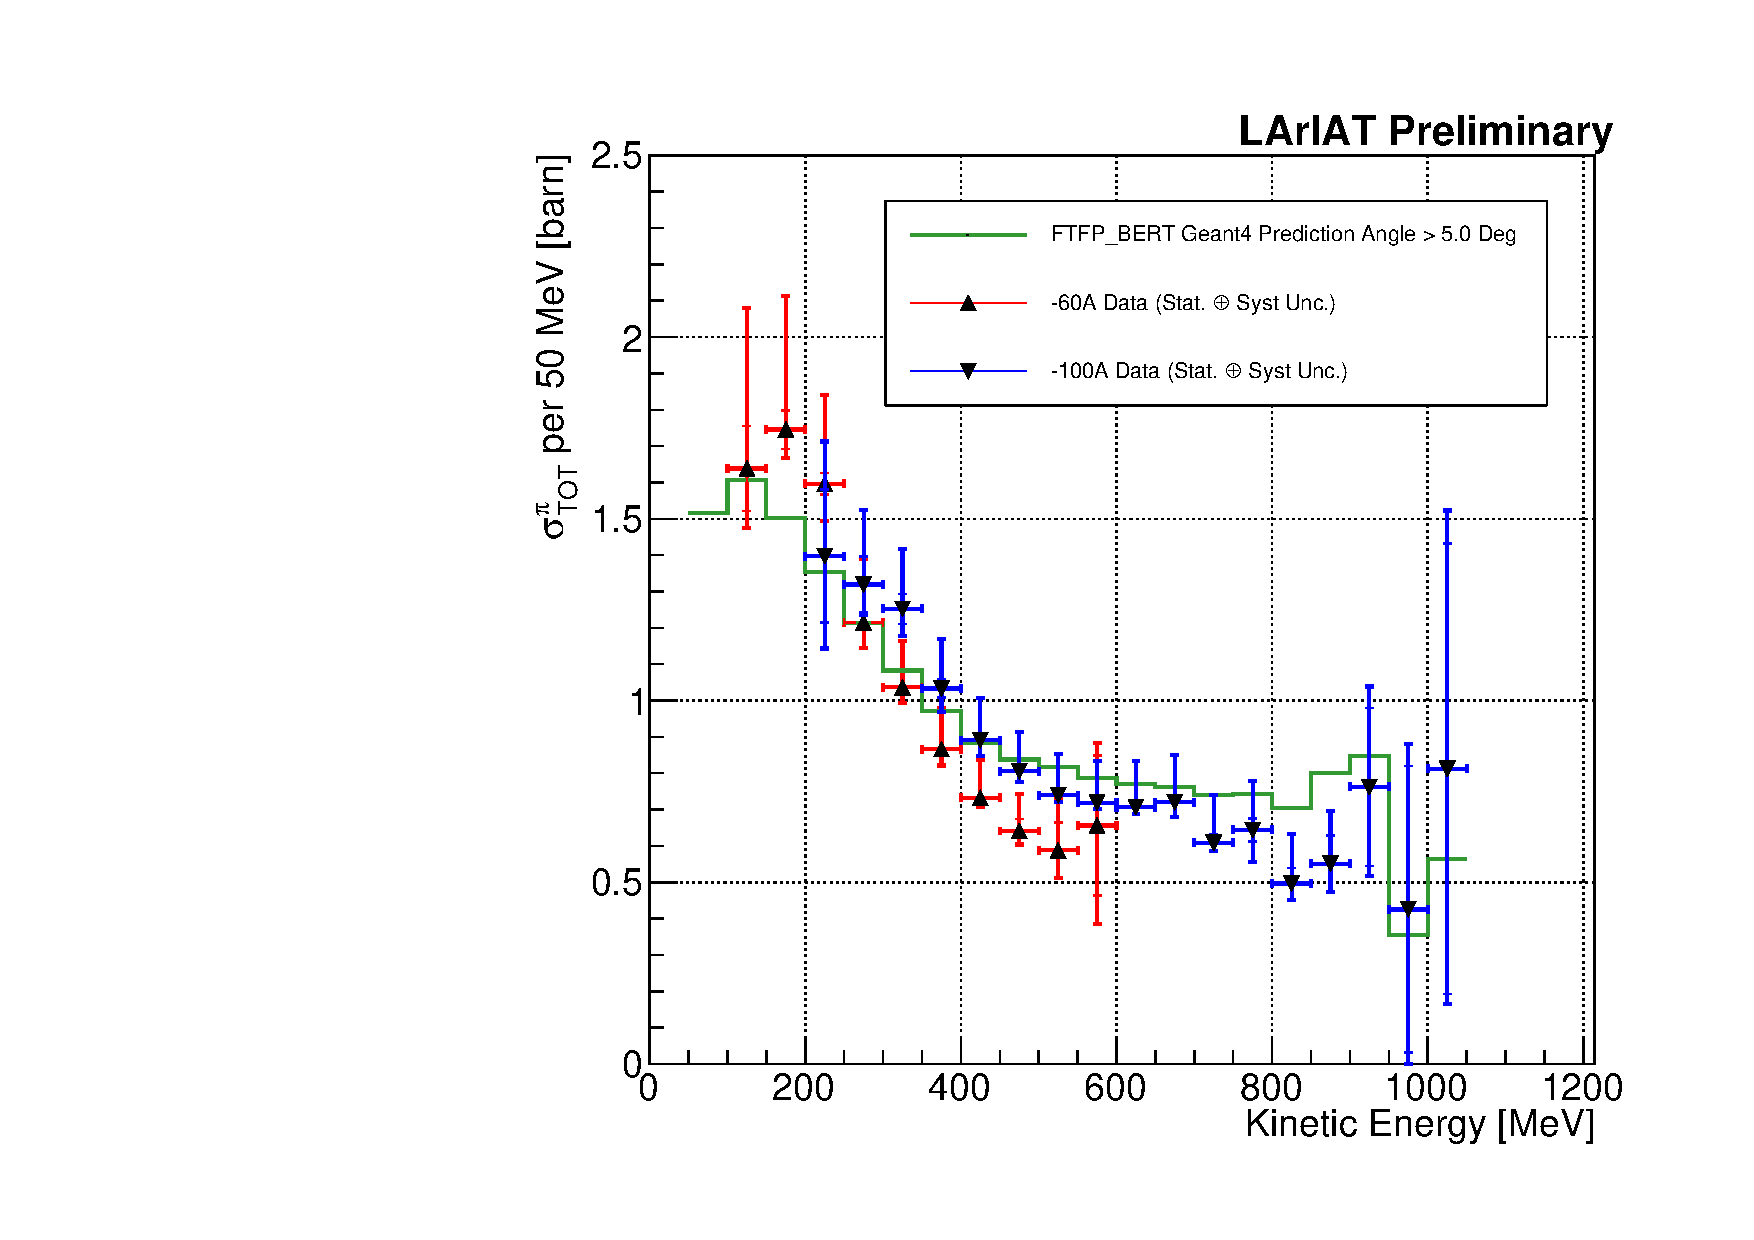
\includegraphics[width=0.48\textwidth]{Chapter-6/Images/TheMoneyPlot.pdf}
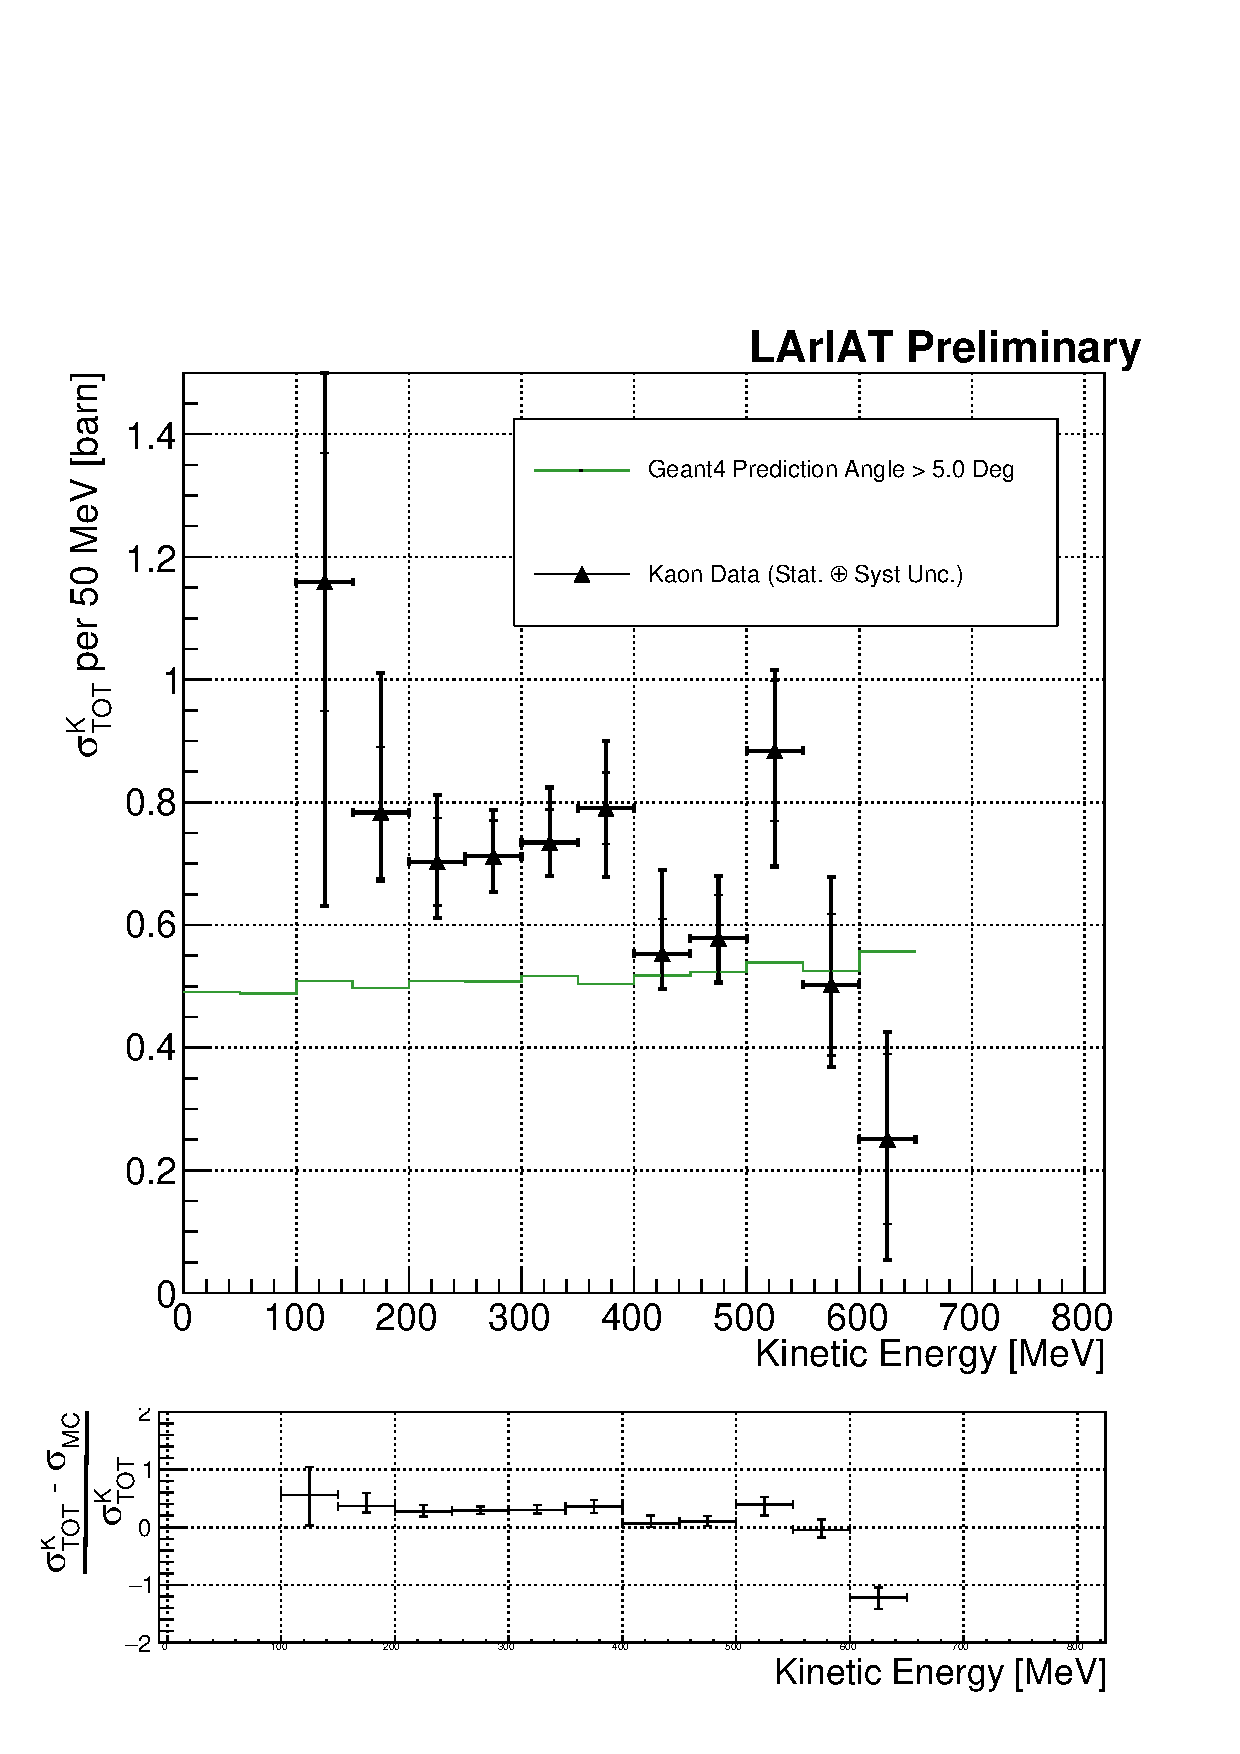
\includegraphics[width=0.48\textwidth]{Chapter-7/Images/TheMoneyPlotK.pdf}
\caption{\emph{Left:} ($\pi^-$-Ar) total hadronic cross section measurements in the 60A and 100A samples overlaid with the  Geant4 prediction (green). \emph{Right:} ($K^+$-Ar) total hadronic cross section for  scattering angles greater than 5$^\circ$ measured in the 60A sample, statistical uncertainty in black and systematic uncertainty in red. The Geant4 prediction for the total hadronic cross section for angle scattering greater than 5$^\circ$ is displayed in green. } 
\label{fig:finalfinal}
\end{figure}


These analyses' will serve as a basis for the future cross section measurements of pions and kaons for the exclusive channels in LArIAT.

